\chapter{Model realization\label{chap:modelReal}}


%Detailed enough to be able to reproduce
%Pseudocode where applicable
%Explain along figure?
%Include technology that's used
%How did we realize/achieve the ideas?

This chapter describes how the concepts presented in chapter \ref{chap:concept} are realized. 
First, some basic design decisions that apply to all realized concepts are described in section \ref{sec:basics}. Section \ref{sec:pairRealization} describes how the concept about pairwise interactions was realized while section \ref{sec:gateRealization} describes the design decisions for the object space concept.
Finally, used and adapted technologies such as the adapted ITM are described in section \ref{sec:technologies}.

\section{Basics \label{sec:basics}}

The following descriptions and assumptions are accurate for all realizations independent of the underlying concept.

\subsection{Single timestep}

One way to learn pushing interactions is to learn the trajectories of entire interactions. While this is possible, for example with a Hidden Markov Model \cite{hmm} and has been done successfully by [TODO look up name] \cite{hmmTrajectory}, it requires labeled training data. More precisely, it requires the models to know when a trajectory starts and when it finishes. Since the model presented here are supposed to learn incrementally by self exploration or at least in an online manner without being provided labeled data from the outside, the models would need to derive the start and endpoints of an interaction automatically. 

The models presented here do not predict entire interactions but rather make small predictions at each timestep in order to avoid the need for such segmentation. This also means that these models are coupled closely to their environment and get updates at each timestep. The actual duration between two updates is not predetermined or restricted by the models presented here. The longer the duration between updates, the more the object states change during an interaction. 
%TODO maybe rearrange the sentences

\subsection{Action primitives}
The action primitives that are available to the model are setting the  two dimensional velocity of the actuator. Due to the environment used, the velocity cannot exceed a norm of $0.5m/s$. Other than that there are no restrictions on the velocity. 
%TODO Maximum velocity is not really relevant to the model, so maybe not really the right place here?

%TODO maybe like this: 
%Similar to the above mentioned timestep, these models assume, that an action is primitive is %selected and performed at each timestep. This results in the assumption that 

\subsection{Used regression and classification model}

In order to meet the goals of incremental lifelong online learning, a regression and classification model is required that allows incremental, local updates. The locality is needed in order to avoid the catastrophic forgetting effect global models experience. As already mentioned in the introduction, this thesis decides to use a memory based model in order to meet these requirements. Unless stated otherwise, all classifiers and regression models, such as the forward model use the adapted ITM described in detail in section \ref{sec:ITM}.


\section{Modeling pairwise interaction \label{sec:pairRealization}}

The pairwise interaction model is based on the interaction space between two objects as already described in the concept chapter \ref{sec:pairInt}. The model itself only operates on interaction features which are computed from the given object states. These features and their computation are detailed in section \ref{sec:intFeatures}. As mentioned above, the model receives a constant stream of updates from its environment regarding the interaction states. Consecutive interaction states are group in \textit{episodes} along with the last action primitive the model executed. 

The naive way for this model to work is to simply store all recorded episodes and perform nearest neighbor search for prediction and planning using equation \ref{eq:bestEpisode}. The simplest norm for $||a,b||_e$ is given by the euclidean norm of the vector resulting from appending $b$ to $a$. However, the euclidean norm assumes all features to be equally important and equally scaled, which is often not the case.




\subsection{Used features \label{sec:intFeatures}}



\section{Object space with gating function \label{sec:gateRealization}}

The realization consists mainly of the parts that are visualized in figure \ref{fig:GateOverview}. 

Algorithm \ref{alg:gatePrediction} shows how a prediction for one object is performed. 


\begin{algorithm}
	\KwIn{Predicted actuator state from action primitive, object state}
	\KwOut{Predicted object state}
	\BlankLine
	relFeature = computeRelativeFeatures(objectState, actuatorState)\\
	\eIf{Gate(relFeatures)}{
		predictedChange = getPrediction(relFeatures) \\
		return add(objectState, predictedChange)
		}{
		return objectState
		}	
	\caption{Prediction pseudocode}
	\label{alg:gatePrediction}
\end{algorithm}

The pseudo function \textit{getPrediction} first selects the responsible forward model before the change is predicted. This selection is being performed based on the identifier of the reference object. If no local model has been trained for the reference object, the predictor tries to find a forward model that is responsible for similar objects. If no suitable forward model can be found, a zero change prediction is returned. This means that the object state remains unchanged.


\subsection{Used features}

This model uses different kind of feature representations. The object states consist of their object specific features. The once that are most important are dynamic features, meaning the features that can actually change. These features are summarized in table \ref{tab:gateObjectFeatures}.

\begin{table}
	\centering
	\begin{tabular}{|c|c|}
		\hline Feature & Description \\ 
		\hline x Position & Global x position in the environment \\ 
		\hline y Position & Global y position in the environment \\ 
		\hline Orientation & Object rotation around the z-axis of the global coordinate system \\ 
		\hline 
	\end{tabular} 
	\caption{Table showing the different dynamic features used to represent objects.}
	\label{tab:gateObjectFeatures}
\end{table}

On top of these dynamic features, static onces like an identifier or information about the shape of the object is included. For example, in order to compute some of the relative interaction features the width and height of the objects are required. Furthermore, the model stores not only the current state of each object but also the previous one. This is required in order to make finite difference estimations about the objects dynamics such as velocity. 
The relative interaction features are summarized in table \ref{tab:gateInteractionFeatures}. 

\begin{table}
	\centering
	\begin{tabular}{|c|c|}
		\hline Feature & Description \\ 
		\hline Id 1 & Identifier of the reference object \\ 
		\hline Id 2 & Identifier of the second object \\ 
		\hline Distance & Closest distance between the two objects \\
		\hline Closing & Describes how much the objects are moving towards each other \\
		\hline Relative x Position & Relative x position of the second object \\
		\hline Relative y Position & Relative y position of the second object \\
		\hline Relative x Velocity & Relative x velocity of the second object \\
		\hline Relative y Velocity & Relative y velocity of the second object \\
		\hline 
	\end{tabular} 
	\caption{Table summarizing the different relative interaction features used to make predictions about interactions. Relative positions and velocities refer to the coordinate system of the reference object.}
	\label{tab:gateInteractionFeatures}
\end{table}

The \textit{Closing} feature $c$ is computed as described in equation \ref{eq:closing} and visualized in figure \ref{fig:closing}.

\begin{equation}
  c = \vec{n} \cdot \vec{rv}
 \label{eq:closing}
\end{equation}

where $\vec{n}$ represents the normal from the reference object towards the second object and $\vec{rv}$ represents the non normalized relative velocity vector of that second object. This equates to the cosine between these two vectors weighted by the magnitude of the relative velocity. This feature is minimal when the second object is moving directly towards the reference object. A positive closing value on the other hand indicates that the objects are moving away from each other. When the feature becomes 0 it indicates that the distance will not change. As mentioned above, the relative velocity is estimated by the finite difference of the current and last position.

The other relative features are computed by transforming their global counterparts to the coordinate system of the reference object. Equation \ref{eq:trans} shows this exemplary for the position:

\begin{equation}
	\vec{relPos} = M \times \vec{gPos}
\label{eq:trans}
\end{equation}

where $M$ is the three dimensional transformation matrix computed from the reference objects orientation and global position. $\vec{gPos}$ is the position vector of the second object extended by a $1$ in order to allow translation along the rotation. 

\begin{figure}
	\centering
	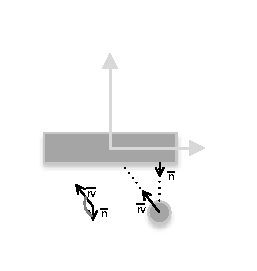
\includegraphics[scale = 1.5]{closing.pdf}
	\caption{Visualization of the closing feature. The gray half circle shows the angle whose cosine is basically computed for the feature.} 
	\label{fig:closing}
\end{figure}

\subsection{Gate}

The gate trains a binary classifier on the relative interaction features about if an interaction takes place or not. 



\section{Used technologies \label{sec:technologies}}

\subsection{Adapted instantaneous topological map \label{sec:ITM}}
%TODO Add pseudo code at the beginning to show general process or nice figure!
%TODO find better name! Consider calling it something closer to kNN since that is kind of what it becomes
The underlying regression and classification model that is used throughout this thesis is an adaptation of the \acrfull{itm} which will be called \acrfull{aitm} throughout this thesis.
The \gls{itm} \cite{itm} is an adaptation of the \gls{gng} \cite{gng} algorithm to create topological maps. Instead of \glspl{gng} global update rules for inserting new nodes in the map, the \gls{itm} uses local update rules in order to be better suited for correlated inputs. 
In order to be applicable to classification and regression, the \gls{itm} was further extended by an output function using the idea of \gls{llm} \cite{LLM}. In order to extend a topological map with an output function, each node represent the corresponding output vector $\vec{w}^i_{out}$ along its input vector $\vec{w}^i_{in}$. The \gls{llm} extends each node further with a local linear mapping $A^i$. This matrix is used to improve the function approximation within each Voronoi cell. With this, the output of each node given an input vector $\vec{x}$ is computed by equation \ref{eq:llmOut}:

\begin{equation}
\vec{y}^i(\vec{x}) = \vec{w}^i_{out} + A^i \cdot (\vec{x}-\vec{w}^i_{in})
\label{eq:llmOut}
\end{equation}

The output function for the net can be computed in multiple ways. The simplest method is to use the output of the winning node, i.e. the output of the node whose input vector $\vec{w}^i_{in}$ is closes to the given input $\vec{x}$. In order to reduce the effect of the metric problem when finding the closest node, the outputs of multiple nodes can also be mixed together. The evaluations in this thesis interpolate the output functions of the two closest nodes:

\begin{equation}
\vec{y}_{net}(\vec{x}) =  \frac{1}{k_n+k_s} \cdot \left[ k_n \cdot \left(\vec{w}^n_{out} + A^n \cdot \left(\vec{x}-\vec{w}^n_{in}\right)\right) + k_s \cdot  \left(\vec{w}^s_{out} + A^s \cdot \left(\vec{x}-\vec{w}^s_{in}\right)\right)\right]
\end{equation}

where $k_n$ and $k_s$ are the weights or importance for the nearest and the second node respectively. These weights are computed as follows:

\begin{equation}
\begin{split}
k_n = \exp\left(\frac{||\vec{x}-\vec{w}^n_{in}||}{\sigma^2}\right) \\
k_s = \exp\left(\frac{||\vec{x}-\vec{w}^s_{in}||}{\sigma^2}\right) 
\end{split}
\end{equation}

$\sigma$ determines the influence radius of each node, just like in radial basis networks \cite{rbf}. The nearest node $n$ and the second closest node $s$ are determined by comparing the input vectors of all nodes in $W$ with the given input vector $\vec{x}$:

\begin{equation}
\begin{split}
	nearest: n = \argmin_{c\in W} ||(\vec{x} - \vec{w}^c_{in})|| \\
	second: s = \argmin_{c\in W\backslash\{n\}} ||(\vec{x} - \vec{w}^c_{in})||
\end{split}
\label{eq:itmNearest}
\end{equation}

During training, the network receives an input-output pair and updates its nodes. First, the two closest nodes $nearest$ and $second$ are computed as stated in equation \ref{eq:itmNearest}. Afterwards, only the node $nearest$ is adapted:

\begin{equation}
\begin{split}
\Delta \vec{w}^n_{in} = \eta_{in} \cdot (\vec{x}^\alpha - \vec{w}^n_{in}) \\
\Delta \vec{w}^n_{out} = \eta_{out} \cdot (\vec{y}^\alpha - \vec{y}^n(\vec{x}^\alpha)) + A^n \cdot \delta \vec{w}^n_{in} \\
\Delta A^n = \eta_A \cdot (\vec{y}^\alpha - \vec{y}^n(\vec{x}^\alpha)) \frac{(\vec{x}^\alpha - \vec{w}^n_{in})^t}{||\vec{x}^\alpha - \vec{w}^n_{in}||^2}
\end{split}
\end{equation}

The initial matrix $A$ is a zero matrix with proper dimensions. The learning rates $\eta_{in}, \eta_{out}$ and $\eta_A$ are meta parameter that need to be determined. In case $\eta_A$ is set to 0, no linear approximation is learned for each Voronoi cell. This means, that each cell has only the constant output of $\vec{w}^n_{out}$.

After the winning node has been updated, the classical \gls{itm} algorithm uses local relations between the new input, the winning node and the second node in order to determine if a new node should be inserted or if some node should be deleted. As long as there are no big jumps in consecutive training samples, this approach works quite well. However, when resetting the environment between consecutive training runs, larger gabs can arise. Furthermore, this network has already been extended by an output function which can now also be used during training. This adapted \gls{itm} inserts new nodes into the network if the current network output varies too much from the target output, i.e if:

\begin{equation}
||\vec{y}^{net}(\vec{x}^\alpha)-\vec{y}^\alpha|| > \epsilon_{ITM}
\end{equation}

The threshold $\epsilon_{ITM} = 10^d$ is dynamically computed, based on the order of magnitude $d$ of the target output norm: %TODO example

\begin{equation}
d = \begin{cases}
\lfloor\log_{10}(||\vec{y}^\alpha||)\rfloor-1 & \text{if $||\vec{y}^\alpha|| > 0$} \\
-k & \text{otherwise}
\end{cases}
\end{equation}

When the output has a norm of $0$ a fixed threshold $10^k$ is chosen. Ideally $k$ should represent the average order of magnitude of the input. This average can be computed incrementally from the non-zero output norms. The benefit of such a dynamic threshold is that it automatically adapts to different use cases. For example, when the \gls{aitm} is used for classification, the output values will be class labels in the form of positive natural numbers. In this case $d=0$ which results in a threshold of 1. In regression tasks however, the output values will be real numbers. It is obvious that different thresholds are required for both types of use case. The \gls{aitm} assumes that the orders of magnitude of the output within one use case are generally rather similar and can be used as an approximation of the desired accuracy.

%TODO Subject to change
With every update the two winning nodes are connected as neighbors. Node deletions are performed just as in the traditional \gls{itm}: Second winners are removed if they are too far away from the winning node. Furthermore, isolated nodes will be deleted. A node is considered isolated if it does not have any neighbors left. Neighbor connections are removed if the second winner in an update can replace a previous neighbor:

\begin{equation}
\forall c \in N(n): \text{If~} (\vec{w}^n_{in}-\vec{w}^s_{in}) \cdot (\vec{w}^c_{in}-\vec{w}^s_{in}) < 0 \text{~remove connection (n,c)}
\end{equation}

$N$ denotes the set of neighbors of the winning node $n$.

\subsection{Abstract inverse model}
%TODO
[TOOD maybe move description from concept here]